\documentclass[answers]{exam}

% packages


\usepackage{etoolbox}
\patchcmd{\thebibliography}
  {\settowidth}
%   {\setlength{\itemsep}{0pt plus 0.1pt}\settowidth}
  {\setlength{\parsep}{0pt}\setlength{\itemsep}{0pt plus 0.1pt}\settowidth}
  {}{}
\apptocmd{\thebibliography}
  {\small}
  {}{}
\usepackage{amsmath}
\usepackage{amsthm}
\usepackage{multirow}
\usepackage[table,xcdraw]{xcolor}
\definecolor{lightgreen}{rgb}{0,0.6,0}
\usepackage{amsfonts}
\usepackage{amssymb}
\usepackage{subfig}
\usepackage[breaklinks]{hyperref}
\makeatletter
\g@addto@macro\UrlBreaks{\do\-}
\makeatother
\usepackage[hyphens]{url}  %% be sure to specify the option 'hyphens'
\hypersetup{
    colorlinks=true,
    linkcolor=blue,
    filecolor=magenta,      
    urlcolor=blue,
    citecolor=blue,
}
\usepackage[format=plain,
            font=it]{caption}
\usepackage{mathrsfs}
\usepackage{graphicx}
\usepackage{caption}
\usepackage{bigints}
\usepackage{enumerate}
\usepackage{outlines}
\usepackage{nicefrac}
\usepackage{datenumber}
\usepackage{listings}
\usepackage{xcolor}
 
\definecolor{codegreen}{rgb}{0,0.6,0}
\definecolor{codegray}{rgb}{0.5,0.5,0.5}
\definecolor{codepurple}{rgb}{0.58,0,0.82}
\definecolor{backcolour}{rgb}{0.95,0.95,0.92}
\definecolor{babyblue}{rgb}{0.54, 0.81, 0.94}
\definecolor{darkseagreen}{rgb}{0.56, 0.74, 0.56}
\definecolor{lilac}{rgb}{0.78, 0.64, 0.78}
\definecolor{mediumlavendermagenta}{rgb}{0.8, 0.6, 0.8}
\definecolor{dandelion}{rgb}{0.94, 0.88, 0.19}
 
\lstdefinestyle{mystyle}{
    backgroundcolor=\color{backcolour},   
    commentstyle=\color{codegreen},
    keywordstyle=\color{magenta},
    numberstyle=\tiny\color{codegray},
    stringstyle=\color{codepurple},
    basicstyle=\ttfamily\footnotesize,
    breakatwhitespace=false,         
    breaklines=true,                 
    captionpos=b,                    
    keepspaces=true,                 
    numbers=left,                    
    numbersep=5pt,                  
    showspaces=false,                
    showstringspaces=false,
    showtabs=false,                  
    tabsize=2
}
\lstset{language=C,keywordstyle={\bfseries \color{blue}}}
 
\lstset{style=mystyle}
% \lstset{style=mystyle}
\usepackage{minted}
\usemintedstyle{vs}

\makeatletter
\renewcommand*\env@matrix[1][\arraystretch]{%
  \edef\arraystretch{#1}%
  \hskip -\arraycolsep
  \let\@ifnextchar\new@ifnextchar
  \array{*\c@MaxMatrixCols c}}
\makeatother

% Title Information

\title{IEMS 394: United States BioFuels Optimisation}
\author{Saif Bhatti, Joyce Lu, Hannah Siegel, Basak Yolac}
\begin{document}

\maketitle
\begin{center}
    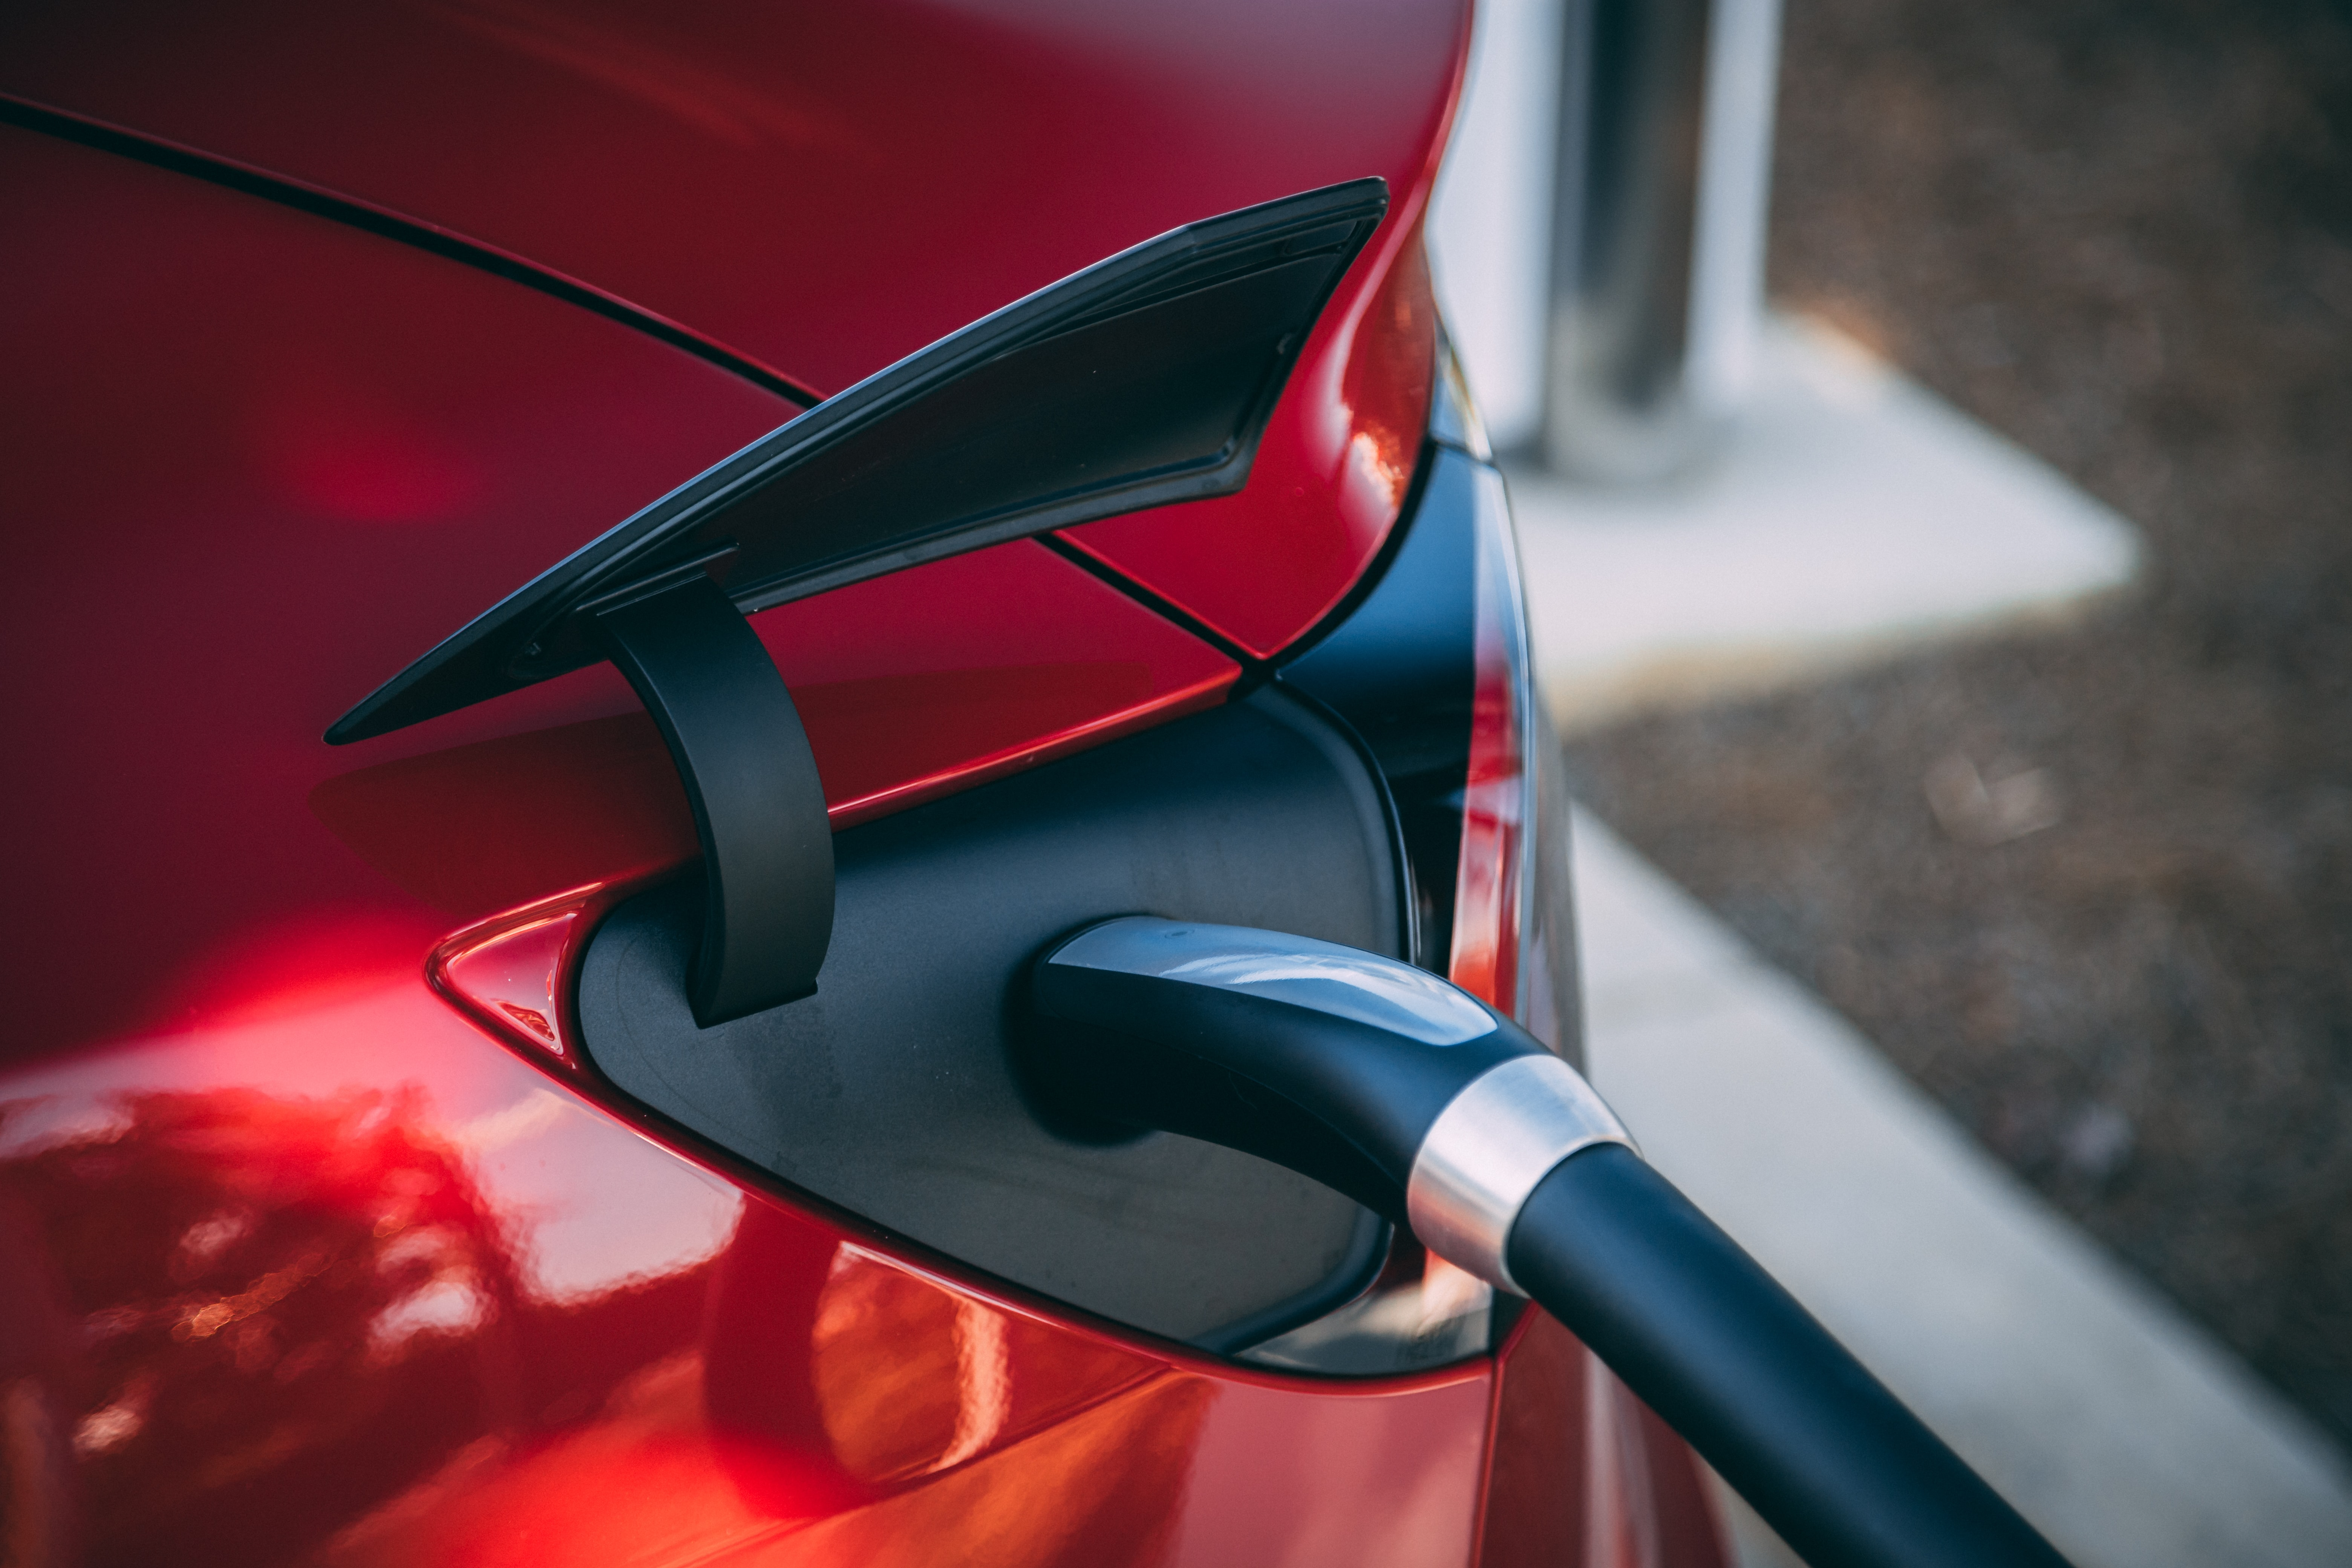
\includegraphics[scale=0.07]{cover.jpg}
\end{center}
\newpage
\section{Introduction}
The internal combustion engine and the use of gas has dominated all types of travel for decades. With E10 gasoline dominating the industry, CO2 emission levels have been at an all time high the past few years\cite{stanford}. While the use of biofuels such as E85 in flex-fuel vehicles have helped to reduce greenhouse gas emissions, there exists a cheaper and cleaner alternative: electric vehicles. Growing consumer demand and infrastructure development have led to the renewed viability of electric vehicles. Figure 1 below shows the tradeoff between buying a gas-run vehicle and an electric vehicle. Electricity costs less than gas but requires more charging time to travel the same distance as a gas car. Furthermore, there are significant differences in pollution and greenhouse gas emissions.

\begin{figure}[h]
    \centering
    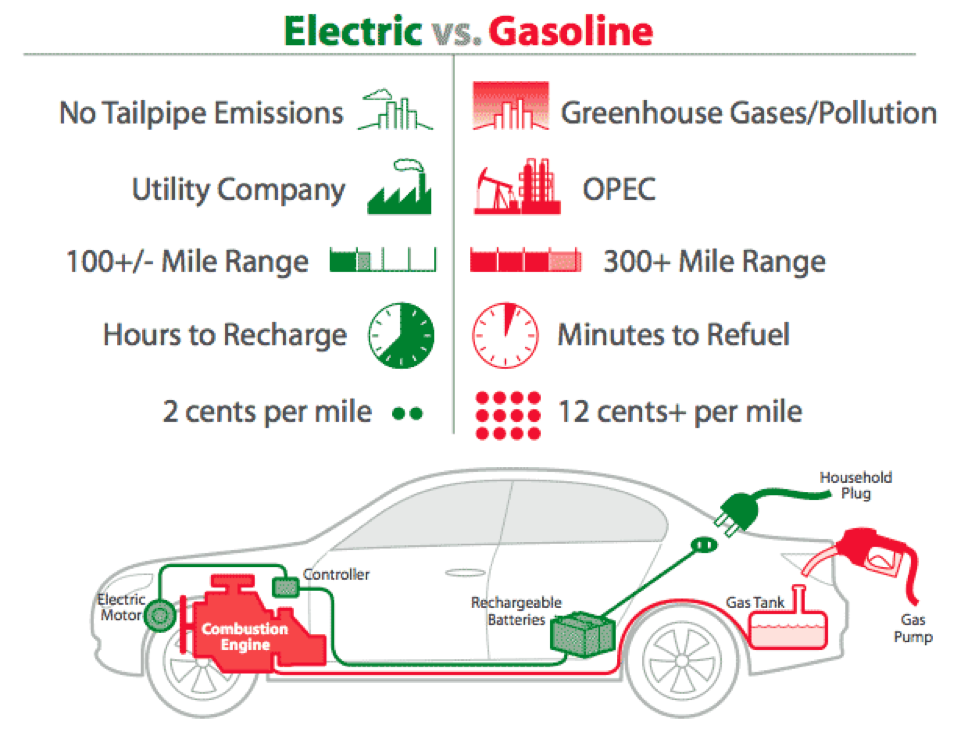
\includegraphics[scale=0.25]{ev_vs_gas.png}
    \caption{Electric vs. Gas Tradeoff\cite{what is an EV}}
    \label{fig:my_label}
\end{figure}
\\~\\
While electrification of light duty fleets in the United States has proven to emit less GHG emissions than both gas and biofuels, the widespread use of electric vehicles is not suitable nor attainable for every county. In particular, this applies to counties with lower rebates, lower population densities and minimal charging capacity. Research of electric vehicle registrations shows that government policy and incentives significantly affect the percentage of people who currently own electric vehicles. If there is a cost incentive to purchase an electric vehicle, this can influence customer decisions. In addition, the research shows that a limited availability of charging stations in a certain county will affect the number of electric vehicles registered in that county. This is also true for biofuels: the amount of flex-fuel vehicles that run on E85 in a given county is dependent on E85 fueling station availability in that county. Research also showed that population density of counties in a state affects vehicle ownership because counties with higher population density may have the capacity for more electric vehicles. A more detailed description of factors that affect electric vehicle, conventional vehicle and flex-fuel vehicle count per county will be discussed in this report.
\\ ~\\
With these considerations in mind, the main task was to build an optimisation model that returns a FFV \footnote{Flex-Fuel Vehicles}/ SIDI ICE \footnote{Spark-Ignition Direct-Injection, Internal Combustion Engine}/ BEV \footnote{Battery Electric Vehicles} split by county as a byproduct of solving for an objective function that seeks to minimise total cost required to adopt this alternative fuel split, with a constraint of reducing statewide GHG emissions by 25 percent. The focus of this model is on minimising total cost of vehicle ownership in three states: California, Minnesota and Texas. These three states were chosen based on variability of government rebates as well as variability in population densities. Moreover, CA has the most extensive infrastructure for EVs and MN has the most extensive infrastructure for E85 use in the United States.

\section{Solution}
\subsection{Optimisation Model}
A python optimisation model was developed using PuLP with the objective of finding the lowest cost combination of BEV, SIDI ICE, and FFV vehicles per county for Minnesota, California and Texas. The model outputs the total minimised cost of vehicle ownership along with following variables:
\begin{outline}
\2 \textbf{n}: the optimal count of each vehicle type per county
\2 \textbf{fc}: the total fuel consumption of the assigned number of each vehicle type per county
\2 \textbf{oc}: the annual operating cost of  the assigned number of each vehicle per county
\2 \textbf{tac}: the total annual cost of the assigned number of each vehicle per county
\2 \textbf{ce}: GHG emissions of the assigned number of each vehicle type per county 
\end{outline}
\\~\\
Set definitions:
\begin{outline}
\2 Let R be the set of counties, using: $r \in R$
\2Let F be the set of vehicle types, using: $f \in F$
\2 Let I be the set of states, using: $i \in I$
\end{outline}
\\~\\
With an objective function to minimise cost to deploy the respective vehicle allocation, the formulation is as follows:
$$\text{min} \sum_{R}\sum_{F}\Big((CF_{rf}\cdot CG_{rf} \cdot CC_{rf})\cdot n_{rf}\Big) \  \forall \ \{r \in R, f \in F\}$$

\begin{outline}
\2 subject to:
\end{outline}
$$ \ \ n_{rf} \geq 0  \  \forall \  r \in R, f \in F$$
$$ce_{rf} = EF_{rf}\cdot n_{rf}  \  \forall \ r \in R, f \in F$$
$$\sum_F ce_{rf}\leq W_r  \  \forall \  r \in R$$
$$n_{rf} \leq \text{e85\_vi}_{r}\cdot T_r \ \forall \ r \in R, f \in F\{\text{FFV}\}$$
$$n_{rf} \leq \text{efuels\_vi}_{r}\cdot T_r \ \forall \ r \in R, f \in F\{\text{BEV}\}$$
$$fc_{rf} = CF_{rf}\cdot n_{rf}\cdot TM_{rf}\ \forall \ r \in R, f \in F$$
$$oc_{rf} = CG_{rf}\cdot fc_{rf} \ \forall \ r \in R, f \in F$$
$$\sum_{f\in F} n_{rf} = T_{r}, \ \forall \ r \in R$$
$$tac_{rf} = oc_{rf} + CC_{rf}\cdot n_{rf} \ \forall \ r \in R, f \in F$$
\\~\\
The solution adheres to emission reduction goals and specific values for total number of assigned vehicles per county, as well as infrastructure constraints on a county-level for BEVs and FFVs. The constraints on the model solution are described in greater detail in the Modelling \& Analysis section and the pseudocode (Appendix A). See Appendix B for model results. 
\newpage
\subsection{Visualisation}
\begin{figure}[h]
    \centering
    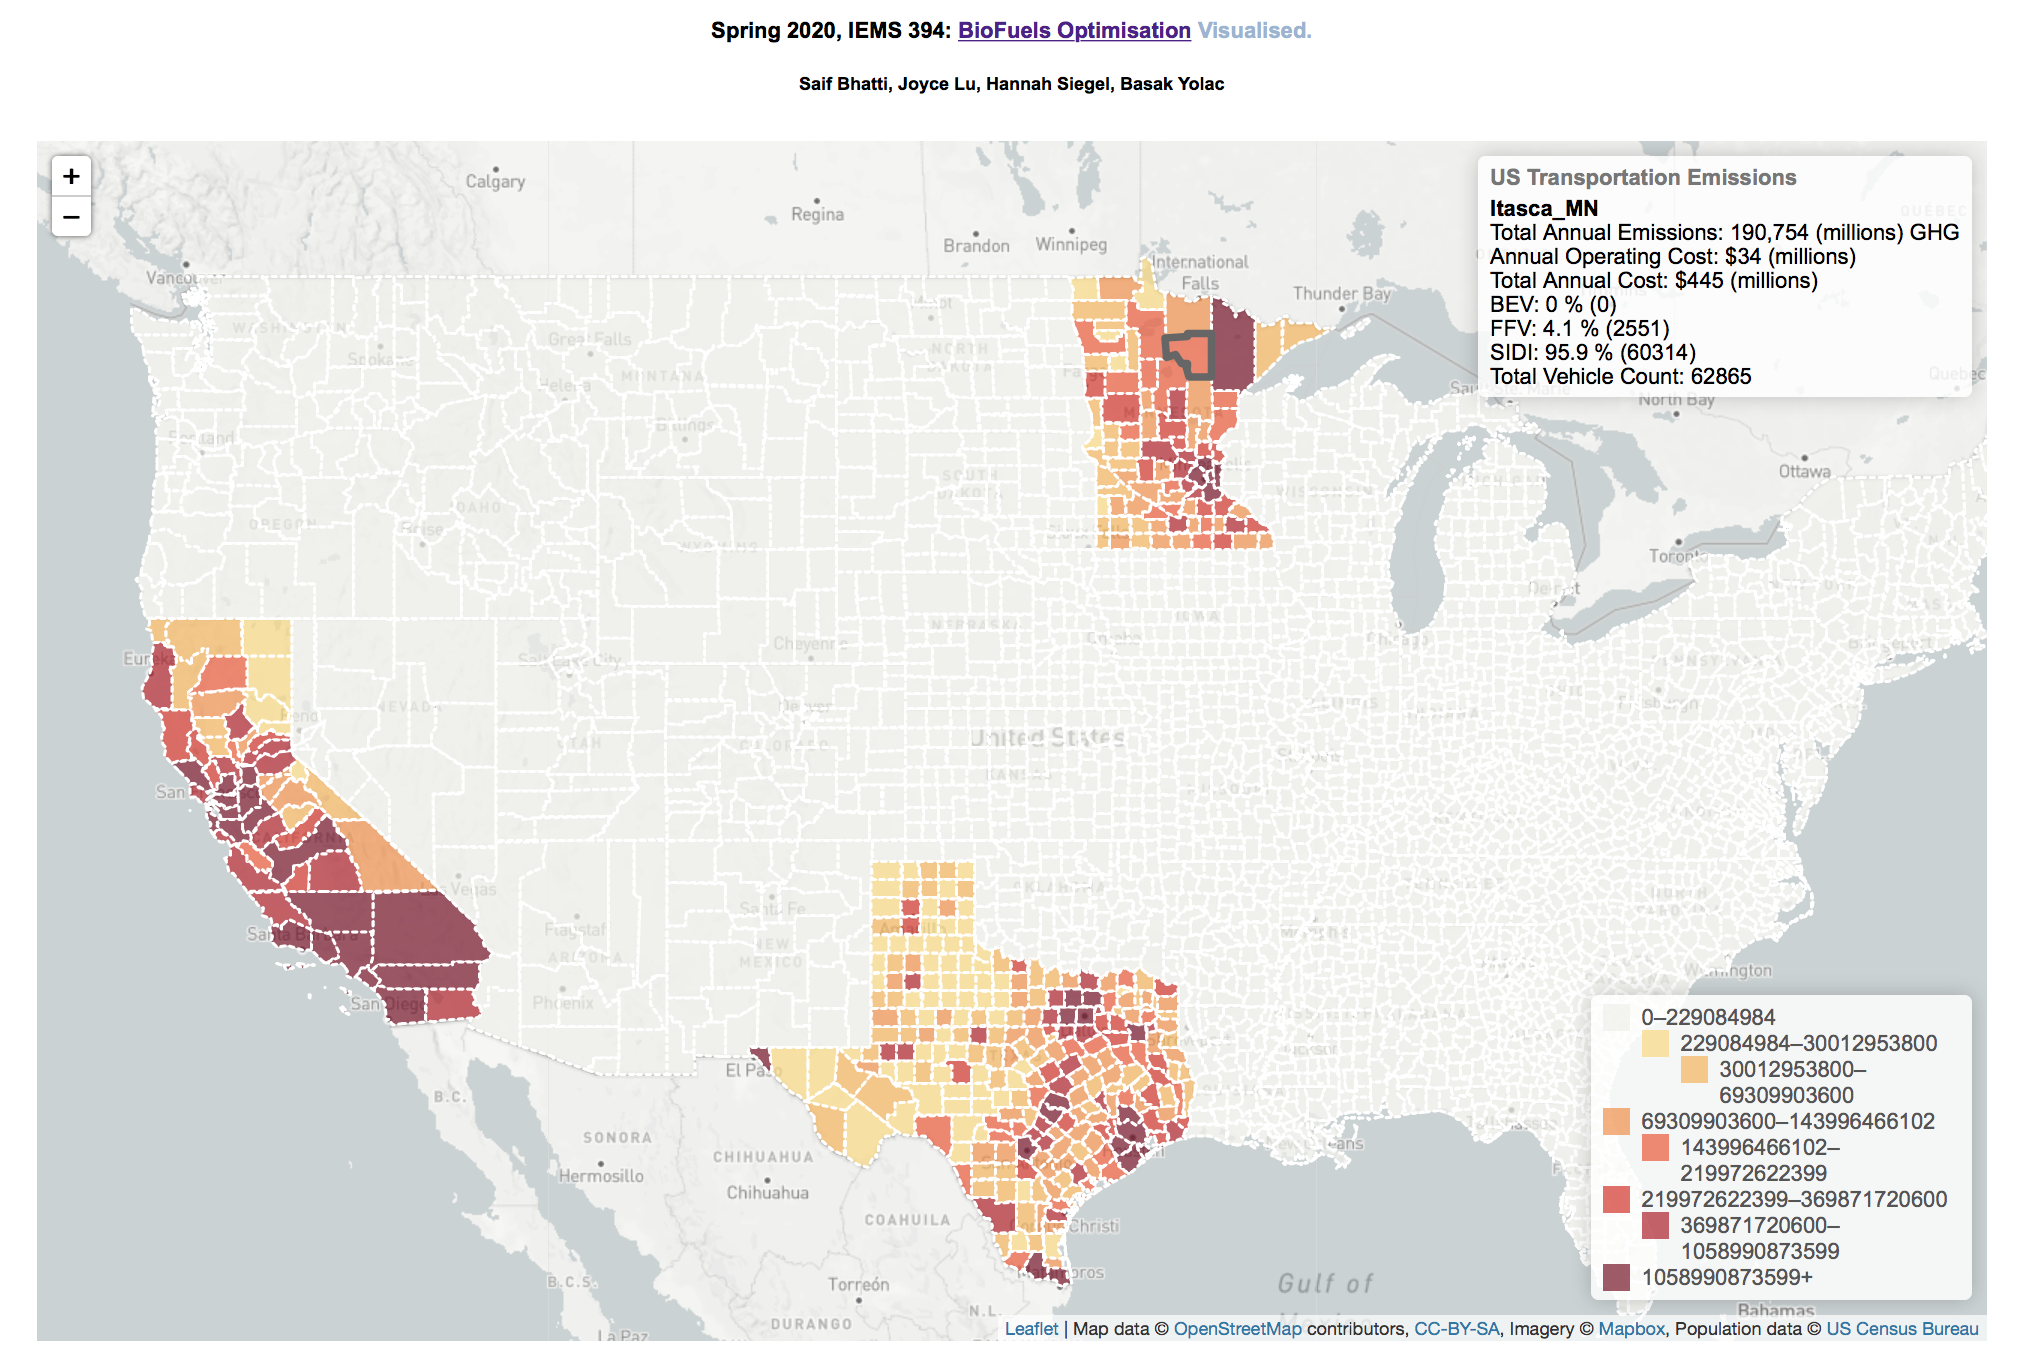
\includegraphics[scale=0.4]{new_visual.png}
    \caption{Visualisation, \href{http://www.saifbhatti.com/iems394}{available online}.}
    \label{fig:my_label}
\end{figure}
\\~\\
The visualisation is built using \href{https://leafletjs.com}{Leafletjs}, and all corresponding data is available on Github. The US counties geo.json file was appended with the results from the optimisation model. This can be loaded as a layer, and then visualised with GHG emissions quantiles that is binned by 10 percentage points.
\\ ~\\
Figure 2 is a visual representation of the model outputs. Darker colors on the map correspond to higher GHG emissions, which is dependent on the number of cars assigned to that specific county, vehicle split recommendations, and emission factors of each vehicle type. Hovering over a county will update the outputs displayed in the top right hand corner. For example, hovering over Itasca MN, the output displays total annual emissions, total operating cost, total vehicle count and vehicle split percentages for Itasca, MN. 

\subsection{Future Development \& Maintenance}
Since the optimisation model primarily uses data from 2019, the client will have to update the data in the future to keep the model up to date. The model takes in CSV files for all the parameters and sets, so the client could easily update any parameter or set by incorporating new data into these CSVs. This way, the data required for the model could be updated without changing the code. Since this model produces results with a single year horizon, producing multi-year analyses requires further development.
\\ ~\\
At this version of the model, viability indexes were created to formulate infrastructure constraints based on existing E85 and EV charging stations\cite{ethanol_fueling_stations}. Therefore, the count of E85 and EV charging stations per county was not included as a parameter. For future development, the number of E85 and EV charging stations could be added as a parameter. This could be an important feature in terms of recommending vehicle fleet splits for hypothetical scenarios consisting of different station counts for EVs and FFVs. This way, the model could be used as a recommendation engine, proposing the number of EV/E85 stations required for the desired vehicle split and their locations.
\\ ~\\
The model could be improved by including data on driving environments in the code, based on the classification of counties as urban, rural or suburban. This information was provided by the client, but including it in the code could provide further analysis on the vehicle fleet of different driving environments, as well as the differences in infrastructure in these areas. This analysis then can be used to improve the charging station analysis. 
\\ ~\\
The scope of the current model only includes the counties in California, Minnesota and Texas. In the future, it could be updated to include all states. Since county-level data on all states was time consuming to capture, the scope was narrowed down. However, the model is designed to work for all states once the necessary information is uploaded. 

\subsection{Assumptions \& Limitations}

Given the relative sparsity of EV and FFV stations, their respective infrastructure is taken into account in the model. However, such considerations were not given to E10 gas stations, and they were assumed available and accessible in every county. While FFVs can run on both E10 and E85, the model is built with a one-to-one mapping between FFVs and E85 fuel. With this assumption, GHG emissions in counties that recommend FFVs may be underestimated. 
\\ ~\\
 The E85 price \cite{E85 Prices}, E10 price, electricity price and emission factor data used in this model is from 2019, and are assumed to not have changed significantly in the past year. While the data on county population is from a 2010 census given by the client, this data was only used to find population density, in which it is assumed that population density does not change significantly from year to year. 
\\ ~\\
Basing electric vehicle registration limitations on existing EV charging station infrastructure originally excluded the fact that people are able to charge their electric vehicles at home. Therefore, it was assumed that in the original model that all electric vehicle charging occurs at charging stations. This will certainly underestimate the recommended EV registrations as it limits the amount of recommended EVs by the accessibility of charging stations. See \textbf{2.5 Updated Assumptions \& Limitations} for further elaboration.
\\ ~\\
California vehicle registration data per county from 2018\cite{cadmv} and Texas vehicle registrations per county from 2017\cite{txdmv} were used in this model.
It is assumed that the number of vehicles from 2017 have not changed significantly. Moreover, county-level vehicle registration data was not available for Minnesota, so the number of vehicle registrations per county was calculated by multiplying the total vehicle registrations in Minnesota\cite{Kaul} by the population density of each county. Therefore, it is assumed that the vehicle registrations are proportional to population density.
\\ ~\\
For the current annual GHG emissions per state, 2016 data was used\cite{US energy info}. It is assumed that the total GHG emissions have not change significantly since 2016. Also, the total GHG emissions data used is specified as emissions by fuel, but it is assumed that they were limited to light duty transportation.


\subsection{Updated Assumptions \& Limitations (September 2020 Update)}

In the original consideration for this research, the EV charging infrastructure was taken as only method by which users could recharge their vehicles. However, this is not accurate, since many users charge their vehicles at their residences. To this end, there are many state-led consumer initiatives to encourage purchase and installation of residential EVSE \footnote{Electric Vehicle Supply Equipment}. As such, this was deemed a central consideration in expanding the EV viability index. 




\section{Supporting Analysis}
\subsection{Research}
In order to quantify GHG emissions for each vehicle type, data was extracted from the ?GREET Model?\cite{GREET} developed by the Argonne National Laboratory. This model uses energy consumption, criteria pollutants, greenhouse gases and water consumption as metrics of sustainability and seeks to simulate the vehicle cycle from vehicle production to vehicle disposal. Emissions factors were computed based on vehicle type and fuel type combinations. From this model, the GHG emission factors were extracted for FFV, SIDI ICE, and BEV vehicles, considering the fuel types they are compatible with. Battery electric vehicles are only compatible with electricity, and in the model conventional vehicles are only compatible with E10 and flex-fuel vehicles are only compatible with E85. This model also supports the fundamental assumption that EVs contribute significantly to any decrease in GHG emissions, as they have an emission factor below half of a conventional gas car equivalent.
\\ ~\\
Electricity price per county, ethanol price per gallon, capital cost of vehicles\cite{electric vs gas cost}, fuel economy of each fuel type and average miles driven with each vehicle type in each county were considered in order to formulate the objective of minimising cost. These were converted to county-level where appropriate and processed either manually or with Python into CSV files. The average miles driven data was found using median income data for each county\cite{national household} and matching that to the data on average miles driven per medium income. 
\\ ~\\
Research shows that not all counties in the U.S. are suitable to have an EV fleet due to insufficiencies in the existing charging station infrastructure. Specifically, counties with minimal charging stations have insufficient conditions for EVs and the use of biofuels in such regions could complement EV fleets in these areas, as suggested by the client. Analyzing the data for charging stations per county, only 1107 counties out of 3100 have EV charging stations. In addition, when plotting charging stations per county by county population, the relationship between the two is very flat and charging stations are insufficient to cover most of the population in some counties, verifying this assumption. Moreover, to explore the existing EV fleet in counties, data on EV registrations per county was found, giving insight into which counties provide necessary conditions to support the use of EVs.  
\\ ~\\
For counties where an EV fleet is infeasible, the model is to allocate between FFV and SIDI-ICE vehicles. However, the allocation of FFVs is further subject to an E85 infrastructure constraint. E85 is 85\% ethanol and is not available at standard gas stations. Across 42 states of the US, there are approximately 3500 fueling stations, so availability must be considered. Finally, E85 is not a substitutable gas in a conventional vehicle and can only be used with FFVs. Despite E85 being a promising clean option to complement an EV fleet, the lack of infrastructure support means it cannot be relied upon nationally.
\\ ~\\
The metrics of EV usage are EV range and MPGe. EV range refers to the distance an EV can travel on a single full battery charge, while MPGe is the distance an EV can travel on the electric equivalent of one gallon of gas. It was decided to use MPGe since it has ubiquitous usage and is more compatible with the data available.
\\ ~\\
To quantify fuel consumption of different vehicle types, the fuel economy projections from the VISION model\cite{vision} were used. The VISION model is a model that uses current data to predict energy use from transportation up to year 2100, including the fuel economy of light duty vehicles. The 2020 average fuel economy is 40.02 MPG for SIDI ICE vehicles, 40.05 MPG for FFVs and 109.08 MPGe for EVs.  
\\ ~\\
The purchase of FFVs and BEVs can be more expensive than conventional cars. However, there are federal and state incentives and rebates that support both biofuels and electric vehicles\cite{state and federal incentives}. There are loan guarantees for the production of biofuels, and production payments to support expanded production of biofuels. In addition, there are research grants from ARPA-E, established under the U.S. Department of Energy, to fund projects that support reducing GHGs, including the use of biofuels and electric vehicles. In addition, ?Alternative Fuel Infrastructure Tax Credit? gives a 30\% tax credit of the cost for fuel equipment. Such incentives promote the use of biofuels and EVs, making them viable at a lower cost. The federal laws and state-level incentives will support the model in terms of the assumptions made for ethanol prices, especially considering the differences in state-level ethanol laws. This data is available for each state, and is provided by the Alternative Fuels Data Center under the U.S. Department of Energy\cite{ethanol laws}. For the model, data on both both state and federal rebates were included. To incorporate the state and federal incentives of BEV and FFV purchases into the model, the rebate amount was subtracted from the capital cost of each vehicle type. 
\\ ~\\
The research paper ?\textit{Transportation options in a carbon-constrained world: Hybrids, plug-in hybrids, biofuels, fuel cell electric vehicles, and battery electric vehicles}?\cite{Sandy}, demonstrates that displacing gas with biofuels and EVs significantly reduces GHG emissions. Their main objective is to simulate the GHG emissions from light-duty vehicles on various fuel types, as shown in Figure 3 below. While cost is not a significant factor in this research, the emission simulation supports the assumption that any combination of biofuels and EVs will cut GHG emissions significantly. Also, this research states that ?No single alternative such as biofuels, a plug-in hybrid or a long-range battery electric vehicle will alone reach our objectives?,  which is why it makes sense to co-deploy biofuels and EVs. There is too much technical and economic uncertainty to claim a single alternative fuel for every region. 

\begin{figure}[h]
    \centering
    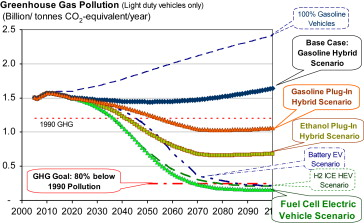
\includegraphics[scale=1]{figure3.jpg}
    \caption{Simulated GHG Emissions}
    \label{fig:my_label}
\end{figure}
\\~\\
Based on the electric vehicle subsidy graphic shown in Figure 4\cite{Jaffe}, the field of interest was narrowed to three states: Minnesota, Texas and California. This selection is based on the spread of electric vehicle adoption in these states. In Minnesota, electric vehicle subsidies are negative. In other words, the capital cost to buy an electric vehicle is higher than an equivalent gas vehicle due to additional taxes. In California, electric vehicles are subsidised at an average tax rebate exceeding \$1000, a result linked to cleaner grid mixtures that vehicles draw from. In Texas, the situation is less coherent across the board, as electric vehicle subsidies are positive in more populous southeastern counties like Harris County, TX and veer towards negative for western counties like Hartley County, TX. 

\begin{figure}[h]
    \centering
    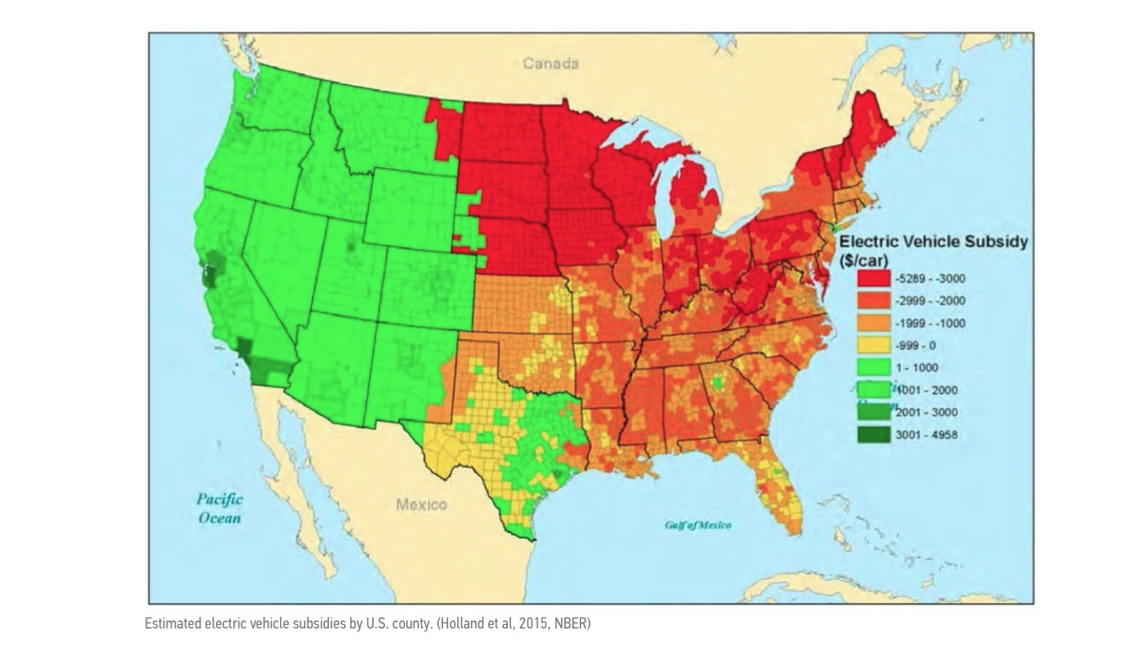
\includegraphics[scale=0.5]{figure4.png}
    \caption{Electric Vehicle Subsidy Map of United States, 2015}
    \label{fig:my_label}
\end{figure}
\\~\\
Since capital costs of vehicles are not usually initially paid in full, the capital cost of each vehicle type was converted to represent what buyers would pay in one year. This was calculated by dividing the capital cost, which equals the upfront cost of the vehicle minus any rebates, by the average time it takes to pay off the vehicle. Average time to pay off EVs is 8 to 9 years\cite{kirby}, and the average time to pay off SIDI ICEs and FFVs is 5 to 6 years\cite{payoff}. Therefore, capital cost minus rebate for BEVs and FFVs were divided by 5.5 and for SIDI ICEs it was divided by 8.5 to normalise the costs.


\subsection{Data \& Software}
\subsubsection{Viability Indices}
Datasets were first converted from excel to csv, and then uploaded to Github for storage and access. Each csv was read into Python as a dataframe, and cleaned using pandas. In some cases, the data did not include county-level data and further manipulation was required. For example, electric vehicle charging stations were provided with only latitude and longitude data. This required downloading US county-level geojson shapefiles, and each point was mapped to a county. The shapely library was used, and this process took extensive time to run ($\sim$40 minutes). This function could be more time efficient through multiprocessing deployment, but due to only requiring a single run per year of EV charging station location data, this was deemed unimportant. In the case of electric vehicle registration, the selected states (MN, TX, CA) were selected from a larger dataset that included data from all states. In this dataset, vehicle registration was provided by zip code data with no field for the county. In order to complete this aggregation, this dataframe was inner-joined with a dataframe containing zip code to county matches. 
\begin{figure}[h]
    \centering
    \subfloat[E85 Fuel Stations]{{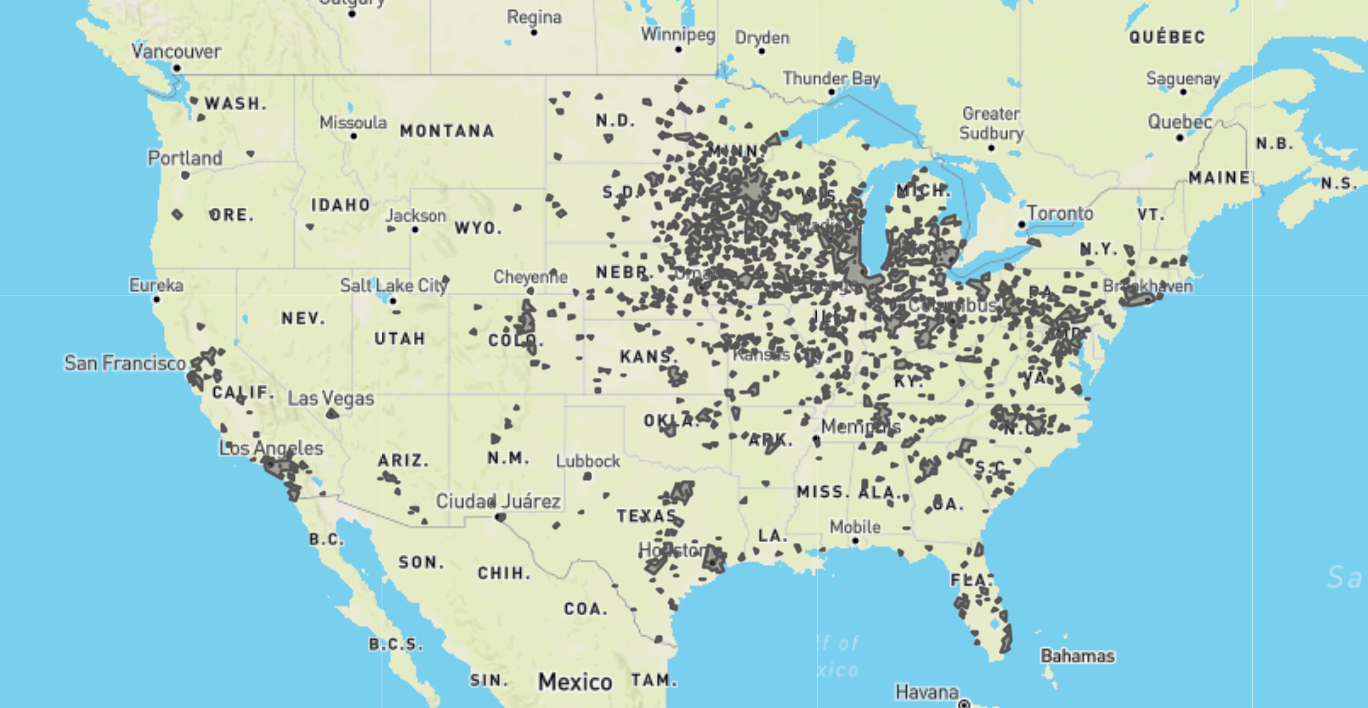
\includegraphics[scale=0.32]{e85_index.png} }}%
    \qquad
    \subfloat[Electric Fuel Stations]{{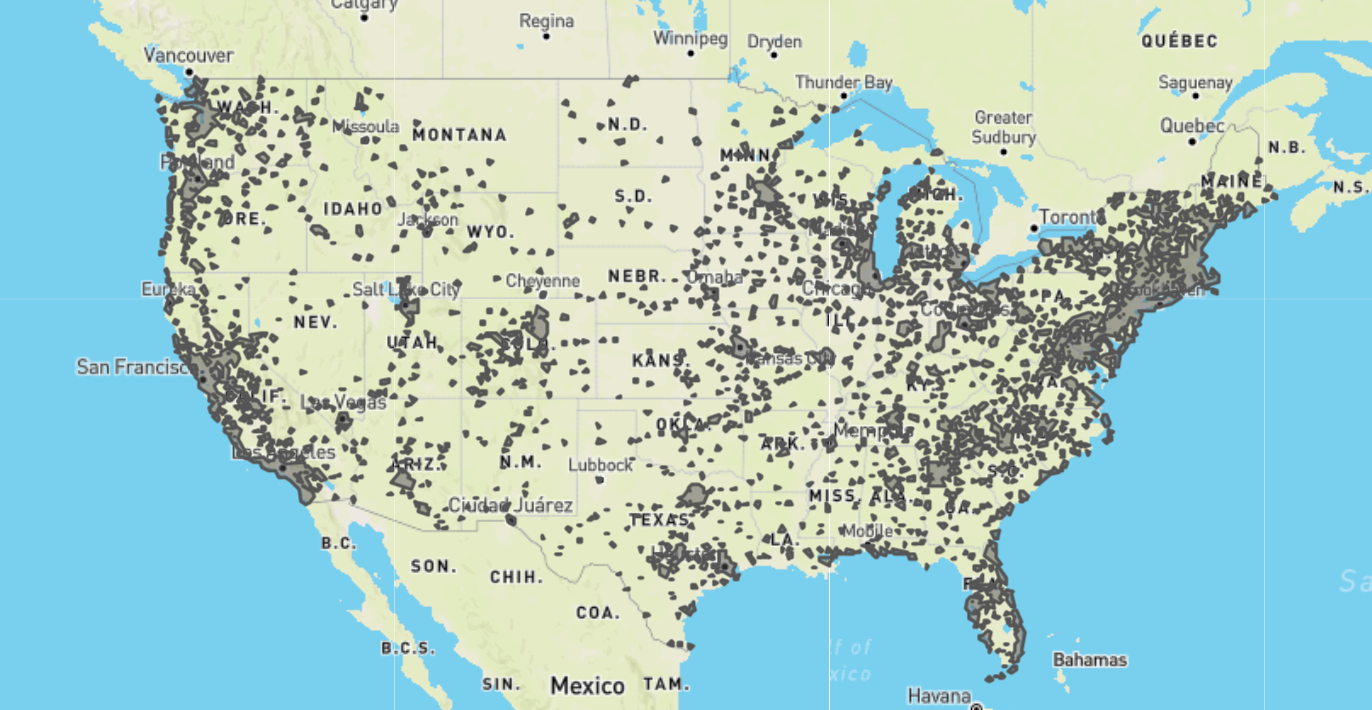
\includegraphics[scale=0.32]{ev_index.png} }}%
    \caption{Visual Representation of Alternative Fuelling Infrastructure in the United States}%
    \label{fig:example}%
\end{figure}
\\~\\
In order to compute indices for E85 and EV charging stations, each station?s position was converted into a driving distance circle. This was to limit the feasibility of assigning either BEV or FFV vehicles to areas where existing infrastructure can support them. The driving distance were conservatively chosen to reflect the relative ubiquity of gas stations as a convenience item, as a 10km or 6.2 mile radius. A cascading union was used to compute the US-wide shape of the respective charging station coverage. By computing a union between the counties shapefile, an index of `county coverage' was found using the following formulation:
$$\text{E85 Viability Index / EV Viability Index} = \frac{\text{E85 / EV covered area}}{\text{Total county area}}$$
The viability indices play a vital role in the development of Constraints 3 and 4, providing a theoretical maximum for FFV / EV capacity in a county. However, despite taking into account the area of a county, these indices do not account for the difference between suburban or rural areas, and urban areas where population and correspondingly vehicle densities will inevitably be higher. For example, if the E85 Viability Index for Cook County is 0.35, then a maximum of 35\% of the vehicles in the county can be flex-fuel vehicles. However, since this 35\% assumes an equal spread, it may heavily underestimate the maximum theoretical in the case that a densely populated city is within this area - in this case the City of Chicago. A further developed index would take population into consideration across zip codes, allowing for more granular analysis that can then be aggregated to the county level.
\\ ~\\ 
Additionally, there is a concern specifically with under-estimation of the EV capacity of a region when only considering public EV charging. Given the fact that E85 is only available at gas stations, this problem does not occur with E85 viability index estimates, which can be taken at face-value. There are few residential EVSE\footnote{Electric Vehicle Supply Equipment} estimates available. In 2010,  the Houston, TX governing body estimated that by 2020, there would be over 1.4 million residential EVSEs across the United States\cite{houston}. It should be noted that this estimation is over 10 years old. However these trends illustrate that clearly more EV owners charge at home - which means any EV viability index which only takes into account the commercial charging station is fallible and will deviously under-estimate charging capacity. Furthermore, commercial charging units have physical limits - they cannot serve infinite cars. In the current formulation, commercial charging stations are being viewed as having infinite server, which is not the case. However, at-home and at-work charging estimations are much closer to 1-to-1 charging ability.
\\ ~\\
In order to address and `even out' this under-estimation, the EV viability index has been altered to include estimates for residential EVSEs. These will not replace existing EV chargers, and thus does results in easing simulated demand for public charging facilities. This is implemented as follows:
\begin{outline}
\1 If a county has a population density exceeding 750 people per square mile, it is considered urban, and an estimated 30\% of its households have access to a residential EVSE. Effective, this county's 
\1 If a county has a population density between 50 and 750 people per square mile, it is considered suburban, and an estimated 40\% of its households have access to a residential EVSE.
\1 If a county has a population less than 50 people per square mile, it is considered rural, and no special estimation is made for residential ESVEs, but public stations remain part of the county's EV viability index.
\end{outline}
\newpage
\subsubsection{Data Pipeline}

In order to run the files, git clone the \href{https://github.com/saif1457/iems394}{iems394 repository} using the following line in terminal:
% \lstinputlisting[language=python]{import os}
\begin{lstlisting}[language=bash, caption=Git Clone]
git clone https://github.com/saif1457/iems394.git
\end{lstlisting}

The entire repository will be downloaded into the specified directory. Next, the user will launch the streamlit application from the command line using:
\begin{lstlisting}[language=bash, caption=Running 394combo.ipynb]
streamlit run publish.py
\end{lstlisting}

Within this application, there are options for tuning model parameters, including the GHG emission goal and driving radii for EV / E85 stations (see top left sidebar). At the time of writing, these are the only two model parameters that can be tuned via the UI, however, full model tuning is available to users by editing either the constituent scripts (.py files). It is worth noting that there are also helpful streamlit docs available \href{https://docs.streamlit.io/en/stable/}{here}. 

\begin{figure}[h]
    \centering
    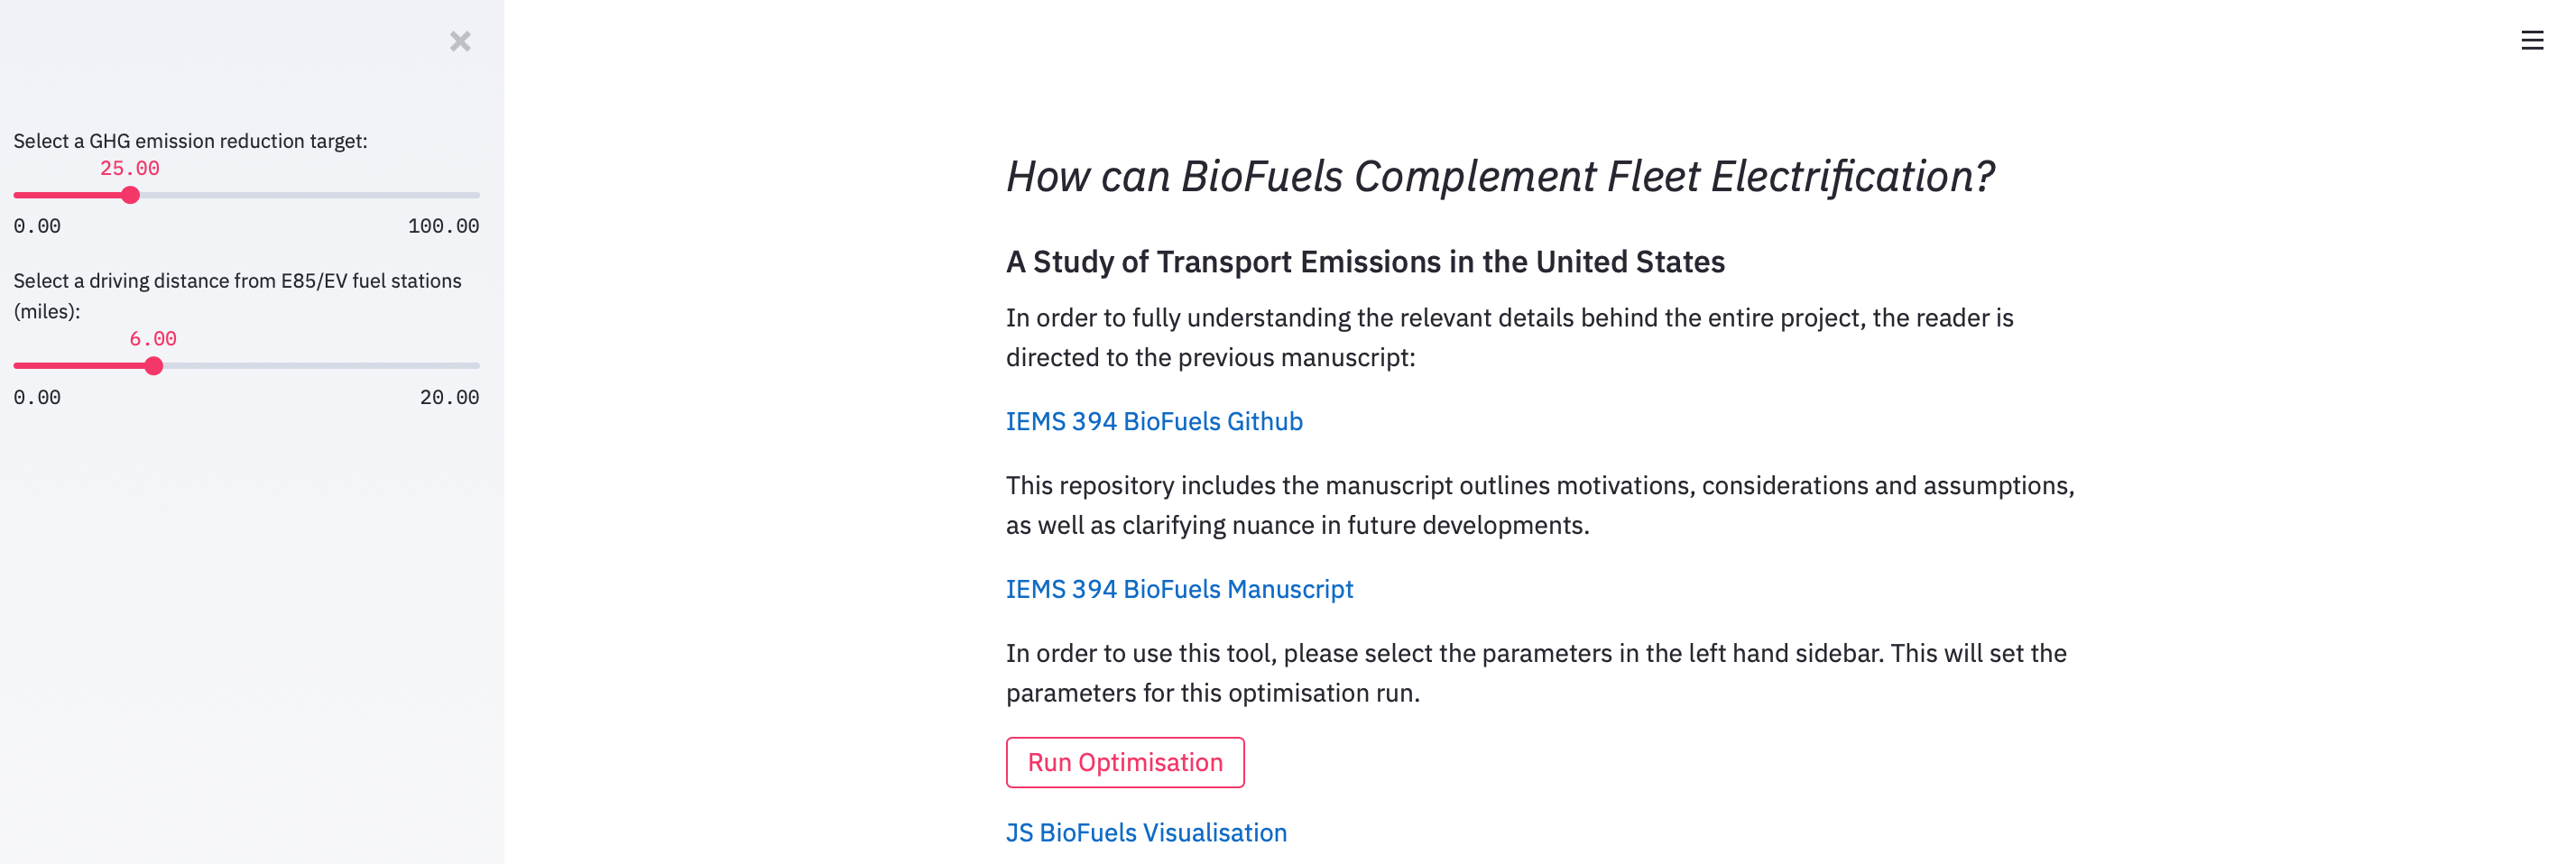
\includegraphics[scale=0.4]{user_options.png}
    \caption{User Options within \textit{394combo.ipynb}}
    \label{fig:my_label}
\end{figure}
\begin{outline}
The order of operations is as follows:
\2\colorbox{dandelion}{preprocessing.py} takes all csv data that needs to be cleaned, and stores it locally in `preprocessed\_data`. Specifically for the Viability Indices, it uses a precomputed value unless the user enters a new value. Runtimes for preprocessed values (6 miles, 10 miles) are near instantaneous, whereas runtimes for new values can be up to `4 minutes`.
\3 Compiling Electric Fueling Stations by county.
\3 Converting zipcode-level data to county-level data.
\3 E85 Fueling Stations and Viability Index Computations.

\2 \colorbox{darkseagreen}{optimisation.py} is the optimisation model which takes in all preprocessed data, and produces an optimised result.
\2 \colorbox{babyblue}{postprocessing.py} takes all optimised output and combines it together into post-processing, producing a \colorbox{mediumlavendermagenta}{state\_output.js} file which updates the \colorbox{lilac}{biofuels.html} visualisation. Running this notebook in its entirety will automatically open the updated visualisation in a new tab.
\\ ~\\
\0 \textbf{Runtime Notes}: 
\2 Pickling is an incredibly useful and tactful technique that avoids unnecessarily re-running swathes of code by instead storing intermediate. To illustrate the point, some useful runtimes include:
\3 Computation of new E85 / EV stations: $>3$ minutes.
\3 Storing processed to disk using pickle: $\sim0.1$ seconds.
\2 Clearly, there is a major runtime improvement from storing data to file after it is computed once. 
\end{outline}
\subsection{Modelling}
The results of the python optimisation model were developed through an objective and the incorporation of various constraints, which constitute the most important part of the model. The main goal of the model is to find the optimal percent allocations of electric vehicles, flex-fuel vehicles, and regular gasoline vehicles that meets the emission reduction goals set by each state at minimum cost. As regular gasoline vehicles are currently the dominant choice of vehicles by far, it is expected that the reallocation will recommend a significant reduction in regular gasoline vehicles and an increase in electric and flex-fuel vehicles. Below are the model constraints and a further exposition on their purpose and rationale. 

\begin{outline}
\1 \textbf{Constraint 0:} The total number of vehicles for each type that are assigned to each county r is a non-negative number. This is necessary because although there is a constraint that requires the sum of vehicles across different types per county to meet a certain threshold, that does not prevent individual counts of vehicles from being negative. 

\1 \textbf{Constraint 1}: Annual emissions of total vehicle counts for each vehicle in each county is equal to the emissions per mile for each vehicle multiplied by the total miles driven for that vehicle type multiplied by the vehicle count. This constraint calculates the annual emissions for each vehicle in each county so that the subsequent constraint to decrease emissions can be implemented. 

\1 \textbf{Constraint 2}: Decrease total emissions by 25 percent. This constraint ensures that emissions of the assigned number of vehicles for all states combined is less than or equal to a 25 percent decrease in current GHG emissions. This constraint sets a limit on the variable \textbf{ce}. 

\0 One of the constraints that the client requested to have in the optimisation model was an infrastructure constraint that reflects maximum electric vehicle and flex-fuel vehicle capacity per county. This is an important constraint, as some counties do not have the infrastructure to support electric vehicles or flex-fuel vehicles either beyond a limit, or at all. This is implemented in Constraints 3 and 4 by limiting the allocation of electric and flex-fuel vehicles based on proximity to available electric and E85 charging stations.

\1 \textbf{Constraint 3}: Infrastructure constraint for E85 based on proximity to an E85 charging station. The total number of flex-fuel vehicles in county r must be less than or equal to a maximum threshold of vehicles. This maximum threshold for county r is computed by multiplying the E85 index by total number of vehicles.

\1 \textbf{Constraint 4}: Infrastructure constraint for EVs based on proximity to an EV charging station, as well as a flat \% boost from residential EVSE charging depending on the population density and classification of a county. For further elaboration on residential EVSE charging, see \textbf{3.2.1 Viability Indices}. The total number of electric vehicles in county r must be less than or equal to a maximum threshold of vehicles. This maximum threshold for county r is computed by multiplying the EV index by total number of vehicles.

\1 \textbf{Constraint 5}: Total annual fuel consumption of each vehicle type per county is equal to the fuel consumption of an individual vehicle of each type multiplied by the number of that vehicle type assigned to each county. This constraint multiples variable n by parameter CF(fuel consumption in gallons/mile of each vehicle type in each county) and then is again multiplied by parameter TM(annual miles driven of each vehicle type in each county). This sets the variable fc to the total annual fuel consumption of each vehicle type per county with units of gallons/year. 

\1 \textbf{Constraint 6}: Operating cost is equal to cost of fuel multiplied by total annual fuel consumption, which was calculated in the previous constraint. Multiplying variable fc by the cost of fuel of each vehicle in each county(in \$/gal) gives the annual operating cost, which is the cost of fuelling each vehicle in each county for one year. 

\1 \textbf{Constraint 7}: Total number of vehicles assigned to each county is equal to the current number of vehicle registrations in that county. This constraint sums the assigned number of each vehicle type for each county and restricts it to the current registration. 
\end{outline}
\subsection{Analysis (September 2020 Update)}
Based on the model outputs and the final visualisation, an overall trend is that GHG emissions are higher in areas that have very high population density, regardless of recommended vehicle type allocation. As shown in Figure 2 above, the darker colors represent larger GHG emissions, and the majority of those counties have high population densities. One overall trend is that GHG emissions are higher in counties that have a very high population density, regardless of recommended vehicle type allocation. This trend appears reasonable because higher population density is proportional to the number of vehicles registered in that county, and thus more vehicles leads to higher emissions. In particular, it is possible that rural counties with low population densities also lack alternative fuel infrastructure, which leads to high SIDI allocation, when compared against suburban and urban counties. When there is a drastic difference in county population densities, vehicle type allocation is less influential in minimising overall GHG emissions. 

\begin{figure}[h]
    \centering
    \subfloat[California]{{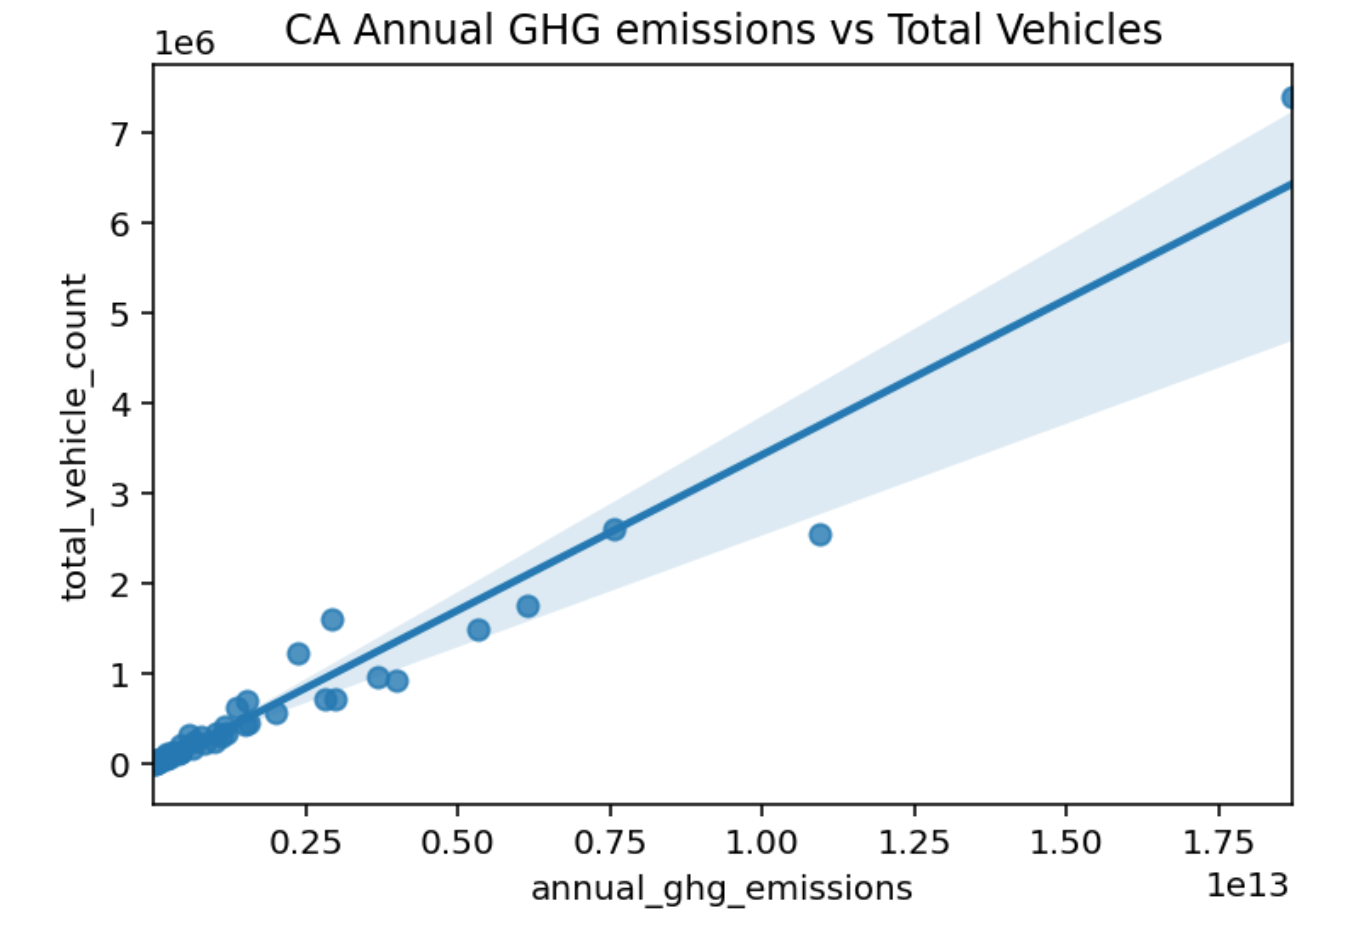
\includegraphics[scale=0.32]{ca_vis.png} }}%
    \qquad
    \subfloat[Minnesota]{{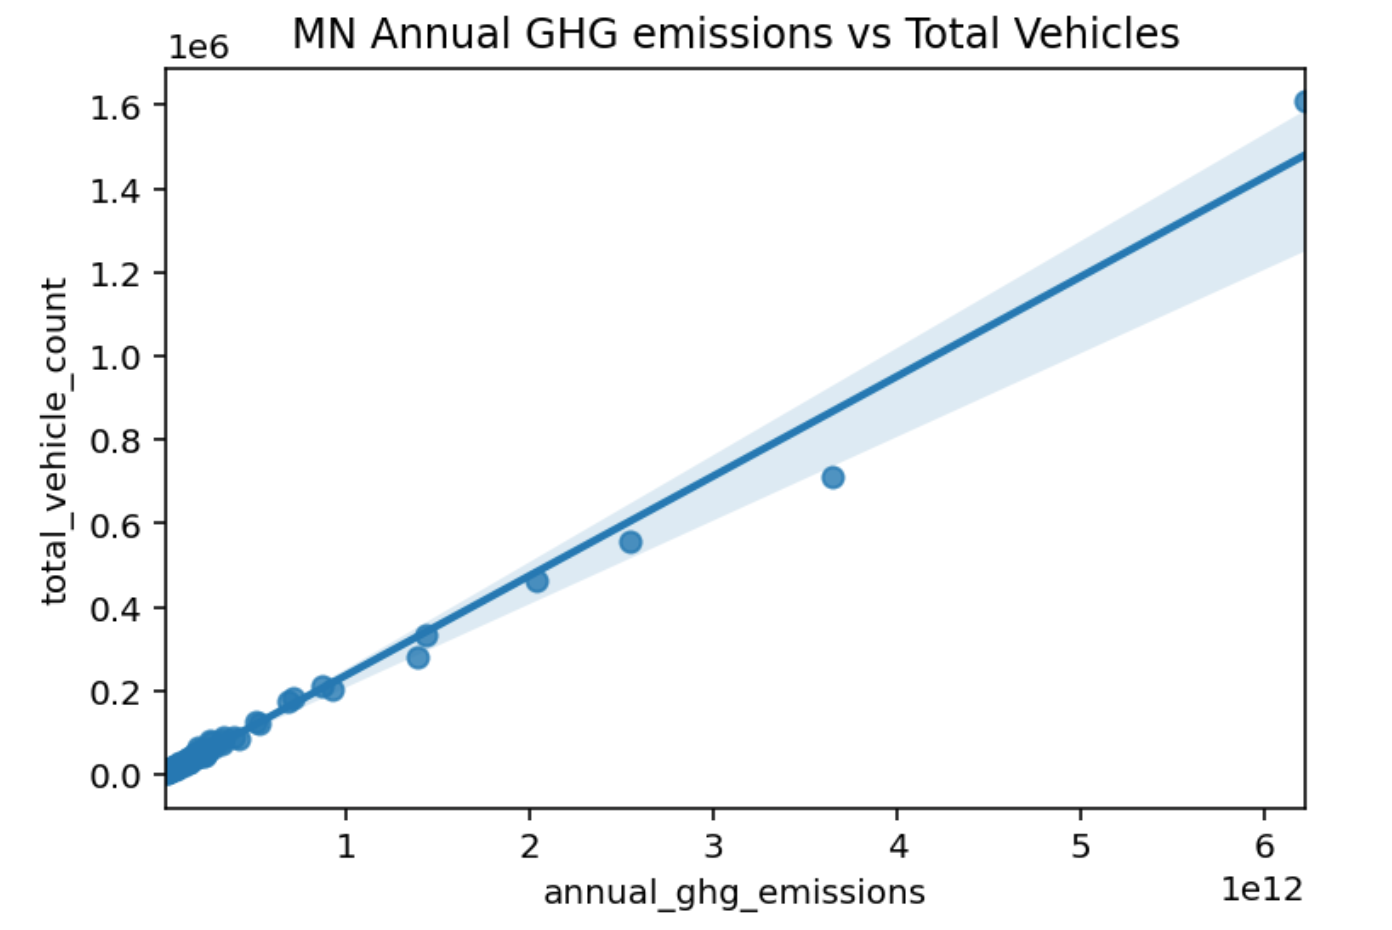
\includegraphics[scale=0.32]{mn_vis.png} }}%
    \qquad
    \subfloat[Texas]{{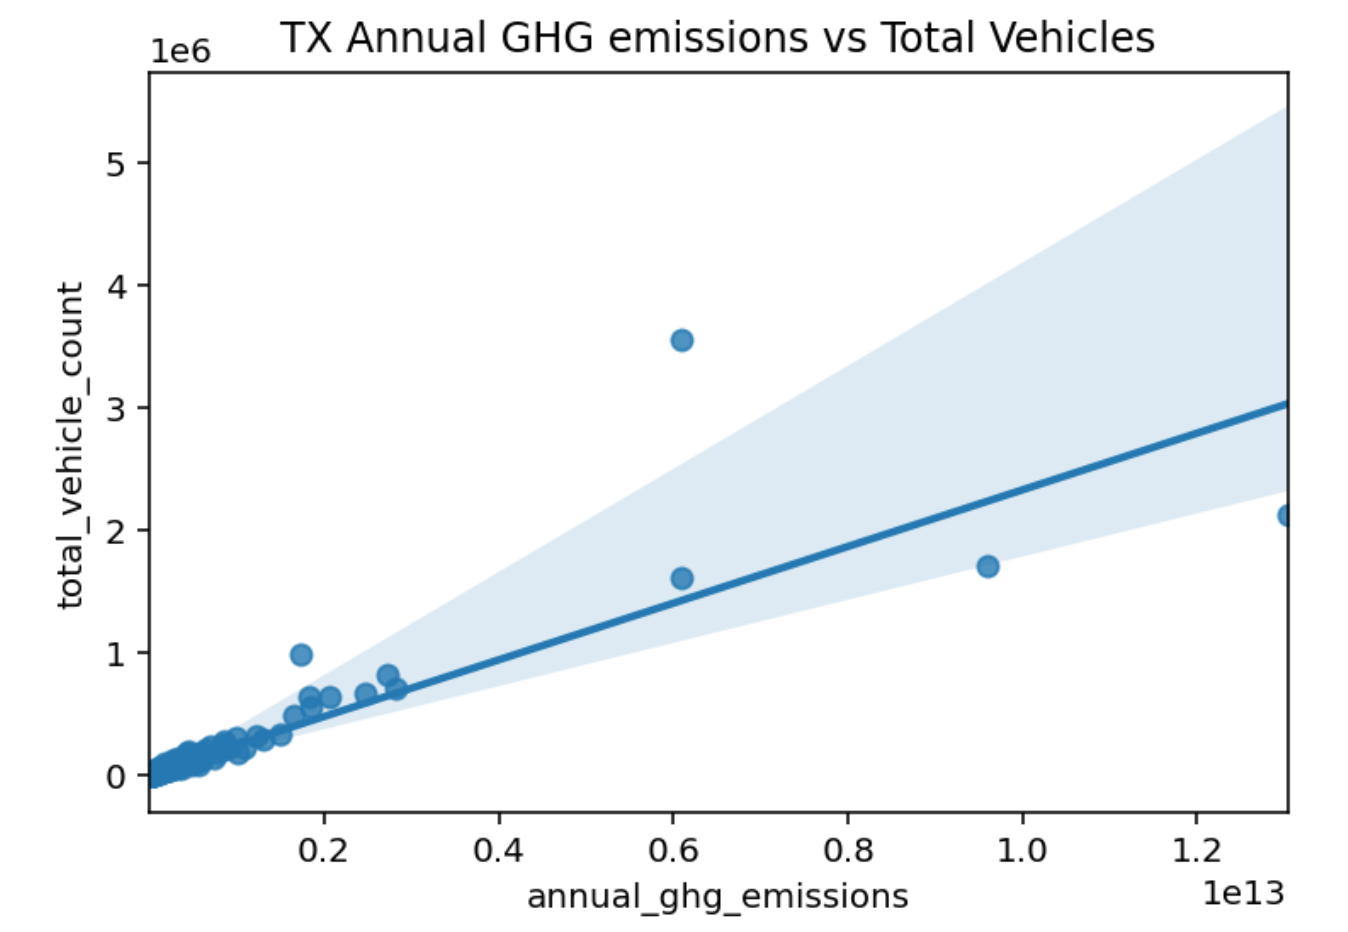
\includegraphics[scale=0.32]{tx_vis.png} }}%
    \caption{Emissions vs. Vehicle Count Trends in the United States}%
    \label{fig:example}%
\end{figure}
\\~\\
Figure 7 (a, b, c) displays the annual GHG emissions based on the recommended vehicle type allocation versus the number of total vehicles allocated to each county, across all three states. This shows that as expected, higher GHG emissions per county are associated with higher vehicle counts in that county. This positive linear trend appears to hold for all three states, with Texas displaying some notable outliers. The clearest such outlier is Harris County, with some $3.5x10^6$ cars, and outputing $6x10^12$ annual GHG emissions. Harris County is home to the City of Houston, and features excellent EV infrastructure as well as some of the country's most generous rebate programs, leading to an optimised result which has a significant alternative fuel allocation: 89.8\% BEV and 10.2\% FFV vehicles.
\\ ~\\
A corollary trend is that counties in rural environments are correlated with higher SIDI allocation recommendations, while counties in urban and suburban environments are correlated with higher BEV and FFV allocation recommendations. The recommended allocation for Modoc, CA - a rural county - is primarily SIDI ICE whereas the recommended allocation in Los Angeles County is exclusive alternative fuel-based (BEV and FFV). Because BEV and FFV allocations were limited by charging station and fuelling station accessibility, this trend appears to fit expectations because stations are less accessible in areas of low population density. Since it is assumed that conventional gas stations can be accessed from every county, those counties that do not support BEVs and FFVs due to viability limits were instead allocated with SIDI ICEs. Since the residential charging emulation was added to the model, there has been a significant uptick in the EV allocation. 
% \begin{figure}[h]
%     \centering
%     \subfloat[BEV comparison]{{\includegraphics[scale=0.32]{bev_diff.png} }}%
%     \qquad
%     \subfloat[FFV comparison]{{\includegraphics[scale=0.32]{ffv_diff.png} }}%
%     \subfloat[SIDI comparison]{{\includegraphics[scale=0.32]{SIDI_diff.png} }}
%     \caption{Comparison Between Allocated Vehicle Percentage vs. Difference in Emissions}%
%     \label{fig:example}%
% \end{figure}
% \\~\\
% Figure 8 displays the comparisons between allocated BEV, FFV, and SIDI ICE percentages and difference in emissions, where difference in emissions is equal to current county emissions minus emissions associated with the recommended vehicle type allocations. Variability in emission reduction appears to increase as the percent allocation of electric vehicles increases, while the same appears to decrease as the percent allocation of flex-fuel vehicles increases. For regular gasoline vehicles, emission reduction variability appears consistent.
\begin{table}[h]
\centering
\begin{tabular}{|c|c|c|c|c|}
\hline
\textbf{State} & \textbf{\begin{tabular}[c]{@{}c@{}}Urban \\ Population \%\end{tabular}} & \textbf{BEV \%} & \textbf{FFV \%} & \textbf{SIDI \%} \\ \hline
\textbf{CA} & 95 & 37.82 & 5.40 & 56.8\\ \hline
\textbf{TX} & 84 & 10.1 & 3.41 & 86.5\\ \hline
\textbf{MN} & 73 & 16.10 & 27.2 & 56.7\\ \hline
\end{tabular}
\end{table}
\\
All three states that were included in the model are mostly urban, and therefore a large portion of the vehicle splits include alternative fuel allocations.There is a slight negative correlation between how rural a county is, and the amount of coverage from pre-established EV charging facilities. In general, \% split of BEVs are larger than that of FFVs due to unavailability of E85 stations compared to EV charging stations. There are more than 21000 charging stations in CA, MN and TX combined as well as residential EVSEs, while there are less than 4000 E85 stations in all of US. Coinciding with expectations based on current infrastructure, Minnesota has the overall highest FFV percent allocation while California has the highest overall BEV allocation.
\\ ~\\
There is a large reduction in the total annual GHG emissions for each state. For CA, there is a 75.17\% decrease, for MN 64.82\% reduction and for TX, there is a 86.40\% reduction. These values are found by comparing the current annual GHG emissions from transportation with annual GHG emissions from the vehicle splits the model suggests. The goal was to decrease the sum of GHG emissions for all three states by 25\% and therefore, the goal is accomplished. 

\subsection{Minnesota}
Of the 87 counties in Minnesota, 18 have no BEV infrastructure (and correspondingly no allocation). As a corollary, these counties are exclusively rural, since both urban and suburban counties have been given an EV boost to account for residential charging. Across these counties, their allocations average 27.4\% FFV and 72.6\% SIDI allocations. There are two counties - Waseca County and Cottonwood County - which boast over 60\% FFV allocations. Of these 18 counties, 15 counties held significant FFV allocations, over 10\%. Other notable counties include:
\begin{outline}
\1 Ramsey County, MN
\2 Ramsey County represents Minnesota's smallest county by census area, but also contains the City of St. Paul, and overall is the second most populous county in Minnesota. Due to its high population density, it has been classified as an urban county, and it also boasts 100\% EV vehicle allocation. 
\1 Hennepin County, MN
\2 Hennepin County represents Minnesota's most populous county, containing the City of Minneapolis. Due to its high population density, it has been classified as an urban county, and also features an entirely alternative fuel allocation with 91.6\% being BEV, and 8.40\% being FFV. 
\1 St. Louis County, MN
\2 St. Louis County is Minnesota's largest county by census area, and is also home to the City of Duluth along its south-eastern boundary. Despite encompassing this urban centre, the rest of the state is very rural, with a correspondingly low population density. Overall - and due in large part to Duluth - the model parameters classify the state as a suburban county. As a result, the +40\% EV coverage boost used to emulate residential EVSEs means that the county now features an increased BEV presence when compared against the original model without this consideration. As a result, St. Louis has a 10.8\% BEV presence. The statewide trend of having extensive biofuels / E85 infrastructure continues, with a 3.60\% FFV vehicle allocation. The remaining 85.6\% is SIDI, which makes sense given the rural nature of upstate St. Louis.
\end{outline}
\subsection{Texas}
Of the 254 counties in Texas, 123 had a non-zero BEV allocation. 
% 661,822,842,664 vs 51,207,579,770
%81,404,209,647,786 vs 6,452,155,051,135 maybe do some kind of \sq analysis (but I dont have time for this)
There are 5 counties in Texas which have FFV allocations where BEV allocations are zero, alluding to the existence of E85 infrastructure where EV infrastructure does not exist. As mentioned previously, these counties have not had an EV coverage boost due to residential charging - which is given only to suburban and urban counties - which means that these counties are rural. Only 2 of these counties - Scurry County and Brown County - accounted for significant FFV allocations (allocations exceeding 10\%), compared with 15 with Minnesota, and none in California in the same analysis. This hints to the relatively limited FFV infrastructure in areas without BEV infrastructure.
\begin{outline}
\1 Dallas County, TX
\2 Dallas County leads Texas in terms of annual GHG emissions by a significant margin (it outputs over 35\% more emissions than second-placed Tarrant County). This is coupled with being home to the City of Dallas, which makes Dallas County an urban county. It comes as a surprise, given this leaderboard, that Dallas County also enjoys one of the nation's more prominent EV rebate programs, which may contribute to its entirely alternative fuel allocation (98.3\% BEV, 1.7\% FFV). There are no SIDI allocations in this county. It is possible that the excess of GHG emissions is representative of the population density, which is also the highest in Texas.
\1 Harris County, TX
\2 Harris County is the second most densely populated county in the state of Texas. It also follows the trend of urban counties in Texas carrying some of the sample's best rebate programs for EVs. As a result, Harris County also boasts 89.9\% EV allocation, with the remaining 10.2\% made up from FFV. 
\1 Bexar County, TX
\2 Bexar county stands out in terms of emissions, and is classed as an `urban' county, containing the city of San Antonio. It has excellent EV infrastructure, which sees 65.70\% of the vehicle allocation assigned as electric. It benefitted significantly from residential enhancements, which took the estimated coverage of EV infrastructure from 65\% coverage to 90.7\%.

\1 Lubbock County, TX
\2 Despite being surrounded by many rural counties in north Texas, Lubbock (TX) boasts existing infrastructure for both EV and E85 fuels. Based on its population density, it is classified as a suburban county, and contains the city of Lubbock. Here, FFV allocations account for almost 30\% of total vehicles (29.40\%), which is more than 10 times the Texas state average of just 3.41\%.
\1 Comal County, TX
\2 Comal County stands out as an anomaly in the Texas alternative fuel landscape, with over 46.1\% of its population rural, it is classified as suburban overall. This leads to the residential EVSE charging boost, and a resultant 41.6\% EV presence. However, the reason for its status as an anomaly is because Comal County is one of few counties across the entire sample to have a higher FFV allocation compared to the BEV allocation where both allocations comprise of high values: (BEV: 41.6\% vs FFV 46.3\%). It also had a 12.10\% SIDI presence. This coupling gives support to the idea that biofuel complements can not only overlap areas that also have a EV infrastructure, but aid in decreasing the SIDI requirements.
\end{outline}

\subsection{California}
Of the 58 counties in California, every single one of them has a non-zero EV allocation, which provides adequate rationale for California to have the highest BEV allocation within this sample of states. In terms of the biofuels complement: there are no counties have a non-zero FFV allocation where BEV allocation is zero. There is despite 29 or 50\% of California's counties having a non-zero FFV allocation. Again, this provides support for the preference for BEV over FFV allocation due to lower emission factors whenever a free choice is available. Even within these 29 counties, average FFV allocation account for only 10.8\% compared against 52.3\% BEV and 36.9\% SIDI.
\begin{outline}
\1 San Francisco County, CA
\2 A clear outlier is San Francisco County and this make sense given that across the analysed states, this is the biggest city/county. San Francisco County (CA) is home to the City of San Francisco, which stands alongside New York and Chicago as the nation's three major urban hubs. Due to being on a peninsula with constrained space (the entire county is only 47 square miles) and the centre of entrepreneurship in the US, it make sense that San Francisco County (CA) has the highest population density in this sample. With the dense county included, the correlation between population density and EV coverage is 0.48, which is moderately positive.

\1 Los Angeles County, CA
\2 Los Angeles County has the highest population density in California, has the highest GHG emissions for the state. The opposite is also true: counties the lowest population densities also have the lowest GHG emissions. For instance, Modoc (CA) is a county with a low population density, and has one of the lowest GHG emissions in the state. This trend is visible despite the fact that Los Angeles (CA) has a (SIDI = 3.2\%, BEV = 63\%, FFV = 33.8\%) split, compared with Modoc (CA) at a (SIDI = 94.7\%, BEV = 5.3\%, FFV = 0\%) split.
\1 San Bernardino County, CA
\2 	Despite being California's largest county by census area, San Bernardino County only registers 9th in terms of GHG emissions. This is mostly due to the lower population density and lack of urban center means that it is classified as a suburban county. Despite having only 4.7\% rural population and benefiting from the EVSE residential charging boost, it only has a 9.9\% EV allocation, 4.3\% FFV allocation and 85.9\% SIDI allocation. This comes as a surprise, and appears to buck the suburban county trend to have significant (over 10\%) EV allocation, but given expansive nature of the county, it also makes sense that lacking sufficient E85 fuel infrastructure means that gas-powered vehicles are more relevant to the possibly longer journeys.  
\end{outline}
\newpage
\newpage
\section{Appendix}
\subsection{Appendix A: Pseudocode}
\subsubsection{Sets}
\begin{outline}
\1 Set are immutable, static dataframes that hold definitions.
\2 V,  	Set of vehicle types \{BEV, SIDI ICE, FFV\}
\2 R,  	Set of counties
\2 S, Set of states \{CA, MN, TX\} 
\end{outline}

\subsubsection{Parameters}
\begin{outline}
\1 Parameters describe objects statically, and is constant in a single simulation. Parameters are only changed to adjust model behaviour.

\2 EF(f, s): Emission factor for fuel type f in state s, (\textit{grams/mile})
\2 CF(v, f): Fuel consumption for vehicle type v using fuel f, (\textit{gallons/mile, or 1/fuel economy})
\2 CG(f, s): Cost of fuel type f in state s, (\textit{\$/gallon})
\2 FE(v, f): Average fuel economy for vehicle type v using fuel f, (\textit{miles per gallon})
\2 CC(v, s): Capital cost, including any rebates, of vehicle type v in state s, (\textit{\$ per vehicle})
\2 D(s): Emission decrease goals per year in state s, (\textit{\%}) 
\2 W(s): Current yearly GHG emissions per state, (\textit{grams})
\2 T(r): Current total number of vehicle registrations per county, (\textit{unit vehicles}) 
\2 TM(v, f, r): Average total annual miles traveled by vehicle v using fuel f in county r, (\textit{miles per year})
\2 N(r): Average income per county, (\textit{\$ per household}) 
\2 B(r, s): Indicates which state s county r is in 
\2 EV(r): Binary variable where 1 if the county location is within a 100 square mile circular range of the nearest EV charging station, 0 otherwise. 
\2 E85(r): Binary variable where 1 if the county location is within a 100 square mile circular range of the nearest E85 station, 0 otherwise. 

\end{outline}
\subsubsection{Variables} 
\begin{outline} 
\1 Variables represent the model state and may change during simulation.
\2 n(v, r): Projected number of vehicles of vehicle type v that should be in county r (\textit{unit vehicles}) 
\2 fc(v, r): Total fuel consumption by vehicle type v in county r, (\textit{gallons per year}) 
\2 oc(v, r): Operating cost of vehicle type v in county r, (\textit{\$ per year})
\2 tac(v, r): Total annual cost of vehicle type v in county r, (\textit{\$ per year})
\2 ce(v, r): Emission by vehicle v in county r, (\textit{grams per year})

\end{outline}
\subsubsection{Constraints}
\begin{outline}
\1 An objective function is optimised with respect to some variables in the presence of constraints on those variables.

\2 \textbf{Constraint 0. Non-negative vehicles assigned to each county r}
\3 Sum of v in Vehicle Types for n(r, v) $>$= 0 for all r in R

\2 \textbf{Constraint 1. Annual emission by total of vehicle v in county f with a given fuel ce(s, r, v) equals emission per mile * total miles driven}
\3 ce(s, r, v) = EF(s, r, v) * n(r, v) for all s in States for r in R for v in V

\2 \textbf{Constraint 2. Decrease total emissions by D(s) for each state r where GHG emissions= total miles by vehicle v per year * emissions per mile}
\3 (Sum of r in Counties, v in Vehicle Types for ce(s, r, v)) $<$= W(s)*(1-D(s)) for all s in S

\2 \textbf{Constraint 3. Infrastructure for E85 based on E85 stations per county. Total number of flex-fuel vehicles in county r is less than the total number of current vehicles when it is within a 100 square mile range of an E85 charging station, if else equal to zero.}
\3 n(r)(v of type FFV) $<$= T(r)*E85(r) for all r in R

\2 \textbf{Constraint 4. Infrastructure for EV based on EV stations per county and estimates for residential EVSE charging. Total number of electric vehicles in county r is less than the total number of current vehicles multiplied by EV}
\3 n(r)(v of type BEV) $<$= T(r)*EV(r) for all r in R

\2 \textbf{Constraint 5. Total annual fuel consumption per county equals fuel consumption of each vehicle (across all types) in that county}
\3 fc(r, v) - CF(r, v)*n(r, v)*TM(r, v) = 0 for all r in R for all v in V

\2 \textbf{Constraint 6. Operating cost is equal to the cost of fuel times sum of fuel consumption for each vehicle type in each county}
\3 oc(r, v) - CG(r, v)*fc(r, v) = 0 for all r in R for all v in V

\2 \textbf{Constraint 7. Total of number of all vehicle types v should be equal to the total of all vehicles in the county }
\3 Sum of v in Vehicle Types for n(r, v) = T(r) for all r in R

\2 \textbf{Constraint 8. Total annual cost is equal to the sum of operating cost and capital cost}
\3 tac(v, r) = oc(v, r) + CC(v, r)*n(v,r) for all r in R for all v in V

\end{outline}
\subsubsection{Objective Function}
\begin{outline}
\1 To minimise the total cost per year driven in all three states (includes the capital cost and operating cost)
\2 Minimise the Sum of v in V across the sum of r in R for CF(r, v)*CG(r, v)*TM(r, v) + CC(r, v)*n(r, v))



\end{outline}
\newpage
\subsection{Appendix B: Model Outputs for Vehicle Count}
See \href{https://raw.githubusercontent.com/saif1457/iems394/master/model_results.csv}{model\_outputs.csv}.
\begin{thebibliography}{99}
\bibitem{stanford} 
Stanford University.``\textit{Global Carbon Emissions Increase}." Stanford News, 17 Dec. 2019, \url{www.news.stanford.edu/2019/12/03/global-carbon-emission-increase/}.
\\
\bibitem{what is an EV}``\textit{Electric Cars: What Is an Electric Car?}" Pacific Coast Electric Heating and Air, 14 Oct. 2015, \url{www.pcelectricheatingandair.com/electric-cars-what-is-an-electric-car}.
\\
\bibitem{ethanol_fueling_stations}
``\textit{Ethanol Fueling Station Locations}.'' Alternative Fuels Data Center: Ethanol Fueling Station Locations, \url{www.afdc.energy.gov/fuels/ethanol_locations.html#/find/nearest?fuel=E85}.
\\
\bibitem{E85 Prices}``\textit{E85 Prices}.", E85 Prices, \url{www.e85prices.com}
\\
\bibitem{cadmv} ``\textit{How Can We Help You Today?}" California DMV, 6 June 2020, \url{www.dmv.ca.gov/portal/}.
\\
\bibitem{txdmv}``\textit{Calendar Year (January - December)}." TXDMV.GOV - Downloads | Calendar Year (January - December) | Vehicles Registered and License Fees by County and Regional Office | Registration Data | VTR | Reports \& Data | Publications, \url{www.txdmv.gov/txdmv-forms/cat_view/13-publications/25-reports-data/65-vehicle-titles-registration/229-registration-data/271-vehicles-registered-and-license-fees-by-county-and-regional-office/272-calendar-year-january-december}.
\\
\bibitem{Kaul} Kaul, Greta, et al.``\textit{The RV Capital of Minnesota, and Other Fun Facts That Can Be Gleaned from Minnesota Vehicle Registration Data}." MinnPost, 5 Sept. 2018, \url{www.minnpost.com/data/2016/07/rv-capital-minnesota-and-other-fun-facts-can-be-gleaned-minnesota-vehicle-registration/}.
\\
\bibitem{US energy info}``\textit{U.S. Energy Information Administration - EIA - Independent Statistics and Analysis}." State-Level Energy-Related Carbon Dioxide Emissions, 2005-2016, \url{www.eia.gov/environment/emissions/state/analysis/}.
\\



\\
\bibitem{GREET} ``\textit{GREET}.? Energy Systems, 2019, Argonne National Laboratory, 2019, 
\url{www.greet.es.anl.gov}.
\\
\bibitem{electric vs gas cost}``\textit{Electric Cars vs. Gas Cars Cost}." Enel X, 7 Oct. 2019, \url{www.evcharging.enelx.com/news/blog/570-electric-cars-vs-gas-cars-cost}.
\\
\bibitem{national household}``\textit{National Household Travel Survey}." National Household Travel Survey, \url{www.nhts.ornl.gov/}.
\\
\bibitem{vision} Maples, John, and Anant Vyas. ``\textit{VISION MODEL}.? VISION Model, Argonne National Laboratory, 2019, 
\url{www.anl.gov/es/vision-model}.
\\
\bibitem{state and federal incentives}``\textit{State and Federal Incentives}." Plug In America - Electric Vehicle Advocacy and Education, 22 Aug. 2019, \url{www.pluginamerica.org/why-go-plug-in/state-federal-incentives/}.
\\
\bibitem{ethanol laws}``\textit{Ethanol Laws and Incentives}." Alternative Fuels Data Center: Ethanol Laws and Incentives, \url{www.afdc.energy.gov/fuels/laws/ETH?state=}.
\\
\bibitem{Sandy}
Thomas, C.E. Sandy. ``\textit{Transportation Options in a Carbon-Constrained World: Hybrids, Plug-in Hybrids, Biofuels, Fuel Cell Electric Vehicles, and Battery Electric Vehicles}." International Journal of Hydrogen Energy, Pergamon, 15 Oct. 2009, \url{www.sciencedirect.com/science/article/abs/pii/S0360319909014980}.
\\
\bibitem{Jaffe} Jaffe, Eric, and CityLab. ``\textit{Mapping Where Electric Vehicles Actually Cause More Pollution Than Gas Cars}." CityLab, 10 July 2015, \url{www.citylab.com/environment/2015/06/where-electric-vehicles-actually-cause-more-pollution-than-gas-cars/397136/}.
\\
\bibitem{kirby} Kirby, Carrie. ``\textit{How Long Does It Take to Break Even With an Electric Car}.? Wise Bread, 22 May 2017, \url{www.wisebread.com/how-long-does-it-take-break-even-with-an-electric-car}.
\\
\bibitem{payoff} ``\textit{6 Ways to Pay Off Your Car Loan Early}." Payoff Life, 18 May 2016, \url{www.payoff.com/life/money/6-ways-to-pay-off-your-car-loan-early/}.
\\
\bibitem{houston}``\textit{Houston, Texas Long Range EV Plan}", 2010. \url{https://www.houstontx.gov/fleet/ev/longrangeevplan.pdf}
\\
\bibitem{news}``\textit{News - MnPASS}." \url{www.dot.state.mn.us/mnpass/mnpassnews.html}.
\\
\bibitem{anna_hecht}
Anna hecht. ``\textit{Car Prices Are Increasing-Here's How That Can Hurt Americans}." CNBC, CNBC, 22 Oct. 2019, \url{www.cnbc.com/2019/10/22/car-prices-are-rapidly-increasing-heres-why-thats-bad-for-americans.html}.
\\
\bibitem{EV benefits}``\textit{Electric Vehicle Benefits}." Plug, \url{www.plugintexas.org/benefits}

\end{thebibliography}
\end{document}\\\\